

\chapter{ElegantBook Writing Sample}

\begin{introduction}
\item Theorem Class Envrionments
\item Cross Reference
\item Math Environments
\item List Environments
\item Logo and Base 
\item $a^2+b^2=c^2$
\end{introduction}


\lipsum[1]
% source: https://www.maths.tcd.ie/~dwilkins/LaTeXPrimer/Theorems.html

\section{Writing Sample}

We will define the integral of a measurable function in three steps. First, we define the integral of a nonnegative simple function. Let $E$ be the measurable set in $\mathcal{R}^N$.

\begin{definition}[Left Coset]
Let $H$ be a subgroup of a group~$G$.  A \emph{left coset} of $H$ in $G$ is a subset of $G$ that is of the form $xH$, where $x \in G$ and $xH = \{ xh : h \in H \}$. Similarly a \emph{right coset} of $H$ in $G$ is a subset of $G$ that is of the form $Hx$, where $Hx = \{ hx : h \in H \} \hbar$ 
\end{definition}

\begin{note}
Note that a subgroup~$H$ of a group $G$ is itself a left coset of $H$ in $G$.
\end{note}

\lipsum[2]

\begin{theorem}[Lagrange's Theorem] \label{thm:lg}
Let $G$ be a finite group, and let $H$ be a subgroup of $G$. Then the order of $H$ divides the order of $G$.
\end{theorem}

As theorem \ref{thm:lg} refered.

\lipsum[3]


\begin{theorem}{theorem name}{label text}
  The content of theorem.
\end{theorem}

we can refer this theorem as \ref{thm:label text}.


\begin{proposition}[Size of Left Coset]
Let $H$ be a finite subgroup of a group $G$.  Then each left coset of $H$ in $G$ has the same number of elements as $H$.
\end{proposition}

\begin{proof}
  Let $z$ be some element of $xH \cap yH$. Then $z = xa$ for some $a \in H$, and $z = yb$ for some $b \in H$. If $h$ is any element of $H$ then $ah \in H$ and $a^{-1}h \in H$, since $H$ is a subgroup of $G$. But $zh = x(ah)$ and $xh = z(a^{-1}h)$ for all $h \in H$. Therefore $zH \subset xH$ and $xH \subset zH$, and thus $xH = zH$.  Similarly $yH = zH$, and thus $xH = yH$, as required. 
\end{proof}

\begin{figure}[htbp]
  \centering
  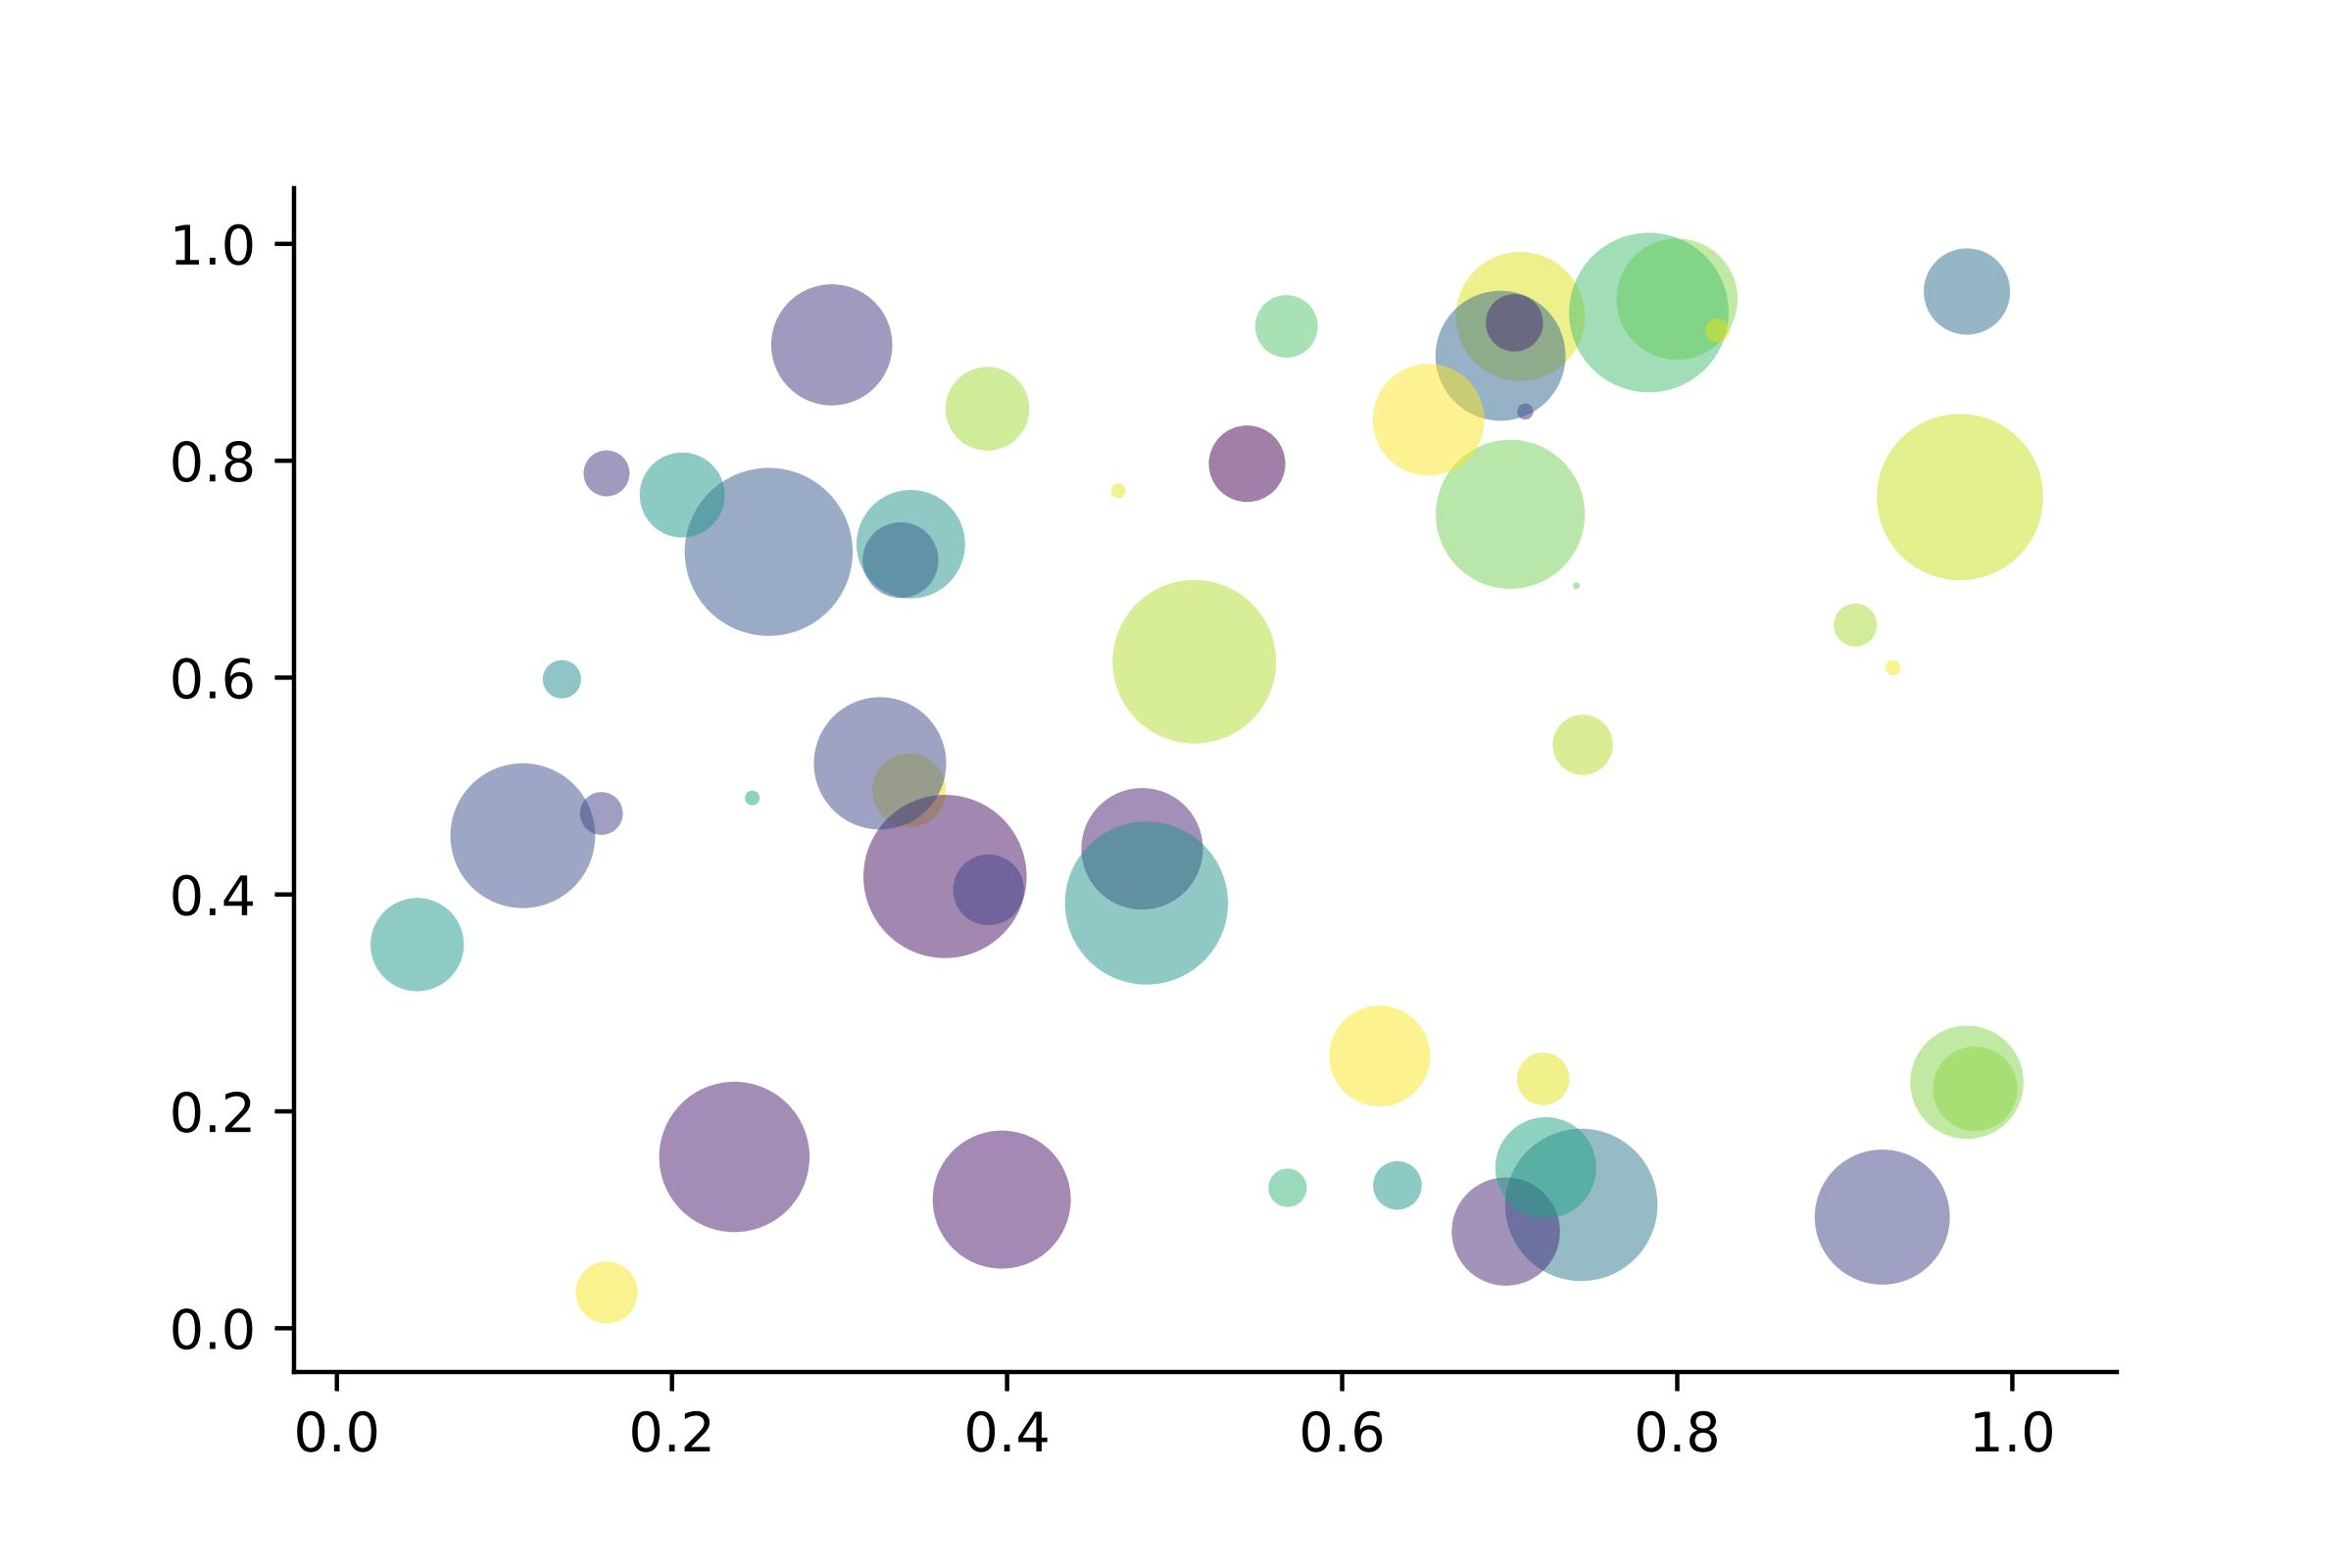
\includegraphics[width=0.6\textwidth]{scatter.jpg}
  \caption{Matplotlib: Scatter Plot Example\label{fig:scatter}}
\end{figure}

Regression analysis is a powerful statistical method that allows you to examine the relationship between two or more variables of interest. While there are many types of regression analysis, at their core they all examine the influence of one or more independent variables on a dependent variable. The process of performing a regression allows you to confidently determine which factors matter most, which factors can be ignored, and how these factors influence each other.

Let's continue using our application training example. In this case, we'd want to measure the historical levels of satisfaction with the events from the past three years or so, as well as any information possible in regards to the independent variables. 

\section{Second section}
This second section\index{S!section} may include some special word, 
and expand the ones already used\index{keywords!used}.


\begin{table}[htbp]
  \small
  \centering
  \caption{Auto MPG and Price \label{tab:reg}}
    \begin{tabular}{lcc}
    \toprule
                    &       (1)         &        (2)      \\
    \midrule
    mpg             &    -238.90***     &      -49.51     \\
                    &     (53.08)       &      (86.16)    \\
    weight          &                   &      1.75***    \\
                    &                   &      (0.641)    \\
    constant        &     11,253***     &       1,946     \\
                    &     (1,171)       &      (3,597)   \\
    obs             &        74         &         74     \\
    $R^2$           &      0.220        &       0.293    \\
    \bottomrule
    \multicolumn{3}{l}{\scriptsize Standard errors in parentheses} \\
    \multicolumn{3}{l}{\scriptsize *** p<0.01, ** p<0.05, * p<0.1} \\
    \end{tabular}%
\end{table}%

\lipsum[1-2]

\begin{itemize}
  \item Routing and resource discovery;
       \begin{itemize} 
             \item Language Models
            \item Vector Space Models
         \end{itemize}
  \item Resilient and scalable computer networks;
  \item Distributed storage and search.
\end{itemize}

%\problemset
\begin{problemset}
  \item Solve the equation $5(- 3x - 2) - (x - 3) = -4(4x + 5) + 13$.
  \item Find the distance between the points $(-4 , -5)$ and $(-1 , -1)$.
  \item Find the slope of the line $5x - 5y = 7$.
\end{problemset}